\question{Схемы включения триода. Динатронный эффект. Тетрод. Пентод}

\subquestion{Схемы включения триода}

Существует три схемы подключения триода с различным положением общей точки: с
общей точкой на катоде (рис.~\pic{22cc}), с общей точкой на сетке
(рис.~\pic{22cg}) и с общей точкой на аноде (рис.~\pic{22ca}).
\vspace{-1.3em}
\begin{figure}[h!]
  \center
  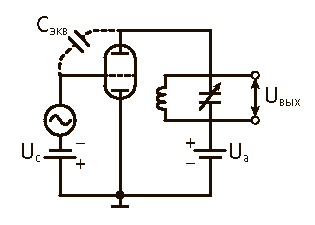
\includegraphics[width=.3\textwidth]{22_common_cathode} \hspace{1em}
  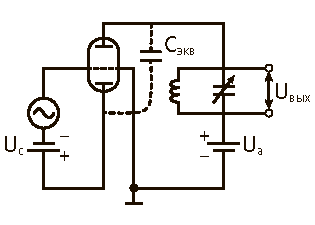
\includegraphics[width=.3\textwidth]{22_common_grid} \hspace{1em}
  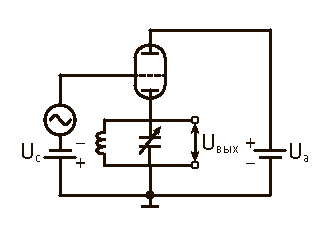
\includegraphics[width=.3\textwidth]{22_common_anode} \\
  \parbox{.3\textwidth}{\caption{Схема включения триода с общим катодом}
    \label{pic22cc}} \hspace{1em}
  \parbox{.3\textwidth}{\caption{Схема включения триода с общей сеткой}
    \label{pic22cg}} \hspace{1em}
  \parbox{.3\textwidth}{\caption{Схема включения триода с общим анодом (катодный
    повторитель)} \label{pic22ca}}
\end{figure}
\vspace{-1.5em}

При небольших частотах подаваемого сигнала \( f < 10^6 \)~Гц чаще всего
используют схему с общим катодом (КПД~\( \sim 85\% \)). В такой схеме
присутствует усиление как по току, так и по напряжению.

Но при частотах \( f > 10^6 \)~Гц на сетке появляется ток смещения, для ее учета
приходится вводить эквивалентную емкость (рис.~\pic{22cc}, штриховая линия).
Через эту емкость часть мощности из выходного контура передается во входной,
приводя к нестабильной работе и самовозбуждению усилителя. Данный эффект
называется \emph{эффектом проходной емкости}.

Для нормальной работы при частотах более 1~МГц используют схему с общей точкой
на сетке, \( C_\text{экв} \) при такой схеме является очень малой. В схеме
отсутствует усиление по току, усиливается только напряжение. Но так как
сетка получается заземленной, то во входном контуре появится ток, в результате
чего усилитель будет иметь более низкий КПД и коэффициент усиления.

Усилительные каскады с общим анодом применяются для усиления импульсов, так как
он вносит малые искажения. Усиления по напряжению нет, но есть значительное
усиление по току.

\subquestion{Тетрод}
Для снижения эффекта проходной емкости между сеткой и анодом ставят
дополнительный электрод~-- экранирующую сетку \( C_1 \) (рис.~\pic{22tetrode}).
На нее подается положительный относительно анода потенциал.
\begin{figure}[h!]
  \vspace{-1em}
  \center
  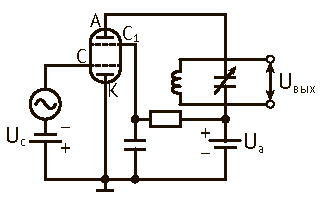
\includegraphics[width=.3\textwidth]{22_tetrode} \hspace{1em}
  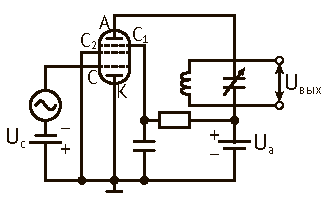
\includegraphics[width=.3\textwidth]{22_pentode} \\
  \parbox{.3\textwidth}{\caption{Схема включения тетрода} \label{pic22tetrode}}
    \hspace{1em}
  \parbox{.3\textwidth}{\caption{Схема включения пентода} \label{pic22pentode}}
  \vspace{-1.5em}
\end{figure}

Недостатком тетрода является \emph{динатронный эффект}. Суть его заключается в
уменьшении анодного тока из-за оседании вторичных электронов, выбиваемых из
анода, на экранирующей сетке, так как она имеет больший, чем у анода, потенциал.
В триоде и диоде такого эффекта не наблюдается из-за того, что анода имеет самый
большой потенциал.

\subquestion{Пентод}

Для устранения динатронного эффекта вводят защитную, антидинатронную, сетку
\( C_2 \) (рис.~\pic{22pentode}), ее заземляют. Между анодом и защитной сеткой
возникает поле, препятствующее попаданию электронов на экранирующую сетку
\( C_1 \).
